\documentclass[11pt,a4paper]{article}

% Packages
\usepackage[margin=1in]{geometry}
\usepackage{graphicx}
\usepackage{booktabs}
\usepackage{amsmath}
\usepackage{amssymb}
\usepackage{hyperref}
\usepackage{enumitem}
\usepackage{caption}
\usepackage{float}
\usepackage{bookmark}

\hypersetup{
    colorlinks=true,
    linkcolor=blue,
    urlcolor=blue,
    citecolor=blue
}

\title{Detecting Patronising and Condescending Language (PCL)\\
Natural Language Processing Coursework Report}
\author{Hardiv Harshakumar (hh1222)}
\date{March 2026}

\begin{document}

\maketitle


\noindent\textbf{GitHub/GitLab Repository:}
\url{https://github.com/hardiv/pcl-detector}

\newpage

% --------------------------------------------------------------------
\section{Exercise 1: Critical Paper Review (Stage 1)}\label{sec:paper_review}

\subsection{Q1. Primary Contributions}
% Q1: Primary contributions of the PCL paper
% - Problem addressed
% - Main methods / resources introduced
% - Key findings
This paper~\cite{perez-almendros-etal-2020-dont} introduces the task of
detecting patronising and condescending language (PCL) in text, particularly in
the context of online news articles about vulnerable communities, which differs
to traditional harmful language detection due to the usually subtler,
well-intentioned and unconscious nature of PCL in this context.

The paper's main contributions include the creation of a novel dataset (Don't
Patronise Me) for PCL detection, which consists of 10,637 paragraphs about
vulnerable social groups selected from news articles annotated for the presence
and type of PCL, both at an overall and a more local text-span level\@.

The paper also establishes experimental baselines across SVM models, BiLSTM
models and fine-tuned transformers such as BERT, RoBERTa and DistilBERT for
binary and multi-label classification of PCL\@.

\subsection{Q2. Technical Strengths}
% Q2: Strengths justifying publication
% - Novelty/originality
% - Soundness of methodology and experiments
% - Significance / impact for the NLP community
The dataset is carefully curated and annotated, and draws from multiple news
sources across 20 countries over a span of 8 years. It employs the Kappa
Inter-Annotator Agreement (IAA) between two annotators (and a third mediating
annotator) to give way to a 5-point scale for labels to address the subjective
nature of identifying PCL\@.

The experimental setup is sound, with appropriate train/dev/test splits and
evaluation metrics.

The baseline RoBERTa model is well-chosen and provides a reasonable starting
point for comparison. With an $F_1$ score of 70.63 on Task 1, it demonstrates
that PCL can be detected, despite its subtlety.

The paper does also identify areas for improvement, such as model failure modes
where knowledge gaps due to world knowledge or commonsense reasoning are
required, and the need for better handling of class imbalance and more
fine-grained PCL types, which can guide future work in this area\@.


\subsection{Weaknesses and Limitations}
% Q3: Weaknesses or insufficient evidence
% - Experimental gaps, missing baselines, lack of ablations, etc.
% - Dataset limitations or potential biases
% - Clarity / reproducibility issues

Whilst care has been taken in the annotation process to avoid subjectivity,
around 14\% of the labels were disagreed upon by the two annotators, which
suggests that the task is inherently subjective and may require more annotators,
as biases and annotation inconsistencies could affect model performance and
generalisability.

In addition, multi-label performance is diminished by severe category imbalance;
the label \"unbalanced power relations\" has 1,307 spans versus only 64 for
\"the poorer, the merrier\", which contributes to near-zero performance on
underrepresented categories. The authors propose using category labels as
privileged information but no ablation or empirical validation of this claim is
provided.

The paper goes on to suggest that BERT-large has overfitted on the small
training dataset, leading it to underperform BERT-base and BiLSTM in Task 1;
this suggestion lacks investigation of regularisation or alternative fine-tuning
strategies to address overfitting.

The paper also lacks formal interpretability analysis, such as SHAP and LIME, to
verify whether the model learns meaningful patterns or is relying on spurious
correlations, which would be useful for understanding model behaviour and
guiding future improvements\@.

% --------------------------------------------------------------------
\section{Exercise 2: Exploratory Data Analysis (Stage 2)}\label{sec:eda}

\subsection{EDA Setup}
All analysis was performed in the Jupyter notebook (\texttt{main.ipynb}) found
in the root of the repository. The labelled corpus comprises the SemEval-2022
train and dev splits of the Don't Patronise Me dataset (10,469 paragraphs in
total). Paragraphs with a graded label $\geq 2$ are treated as PCL-positive;
those with labels 0--1 are PCL-negative. No tokeniser-specific preprocessing was
applied during EDA\@; a simple lower-cased alphabetic-token regex was used for
vocabulary and n-gram statistics to remain model-agnostic.

\subsection{Technique 1: Statistical Profiling}

\subsubsection{Visual/Tabular Evidence}

Table~\ref{tab:vocab_stats} summarises vocabulary size, token count, and
type-token ratio (TTR) for each class. Figure~\ref{fig:wordcount} shows the
distribution of paragraph lengths in words, annotated with the 95th and 99th
percentiles.

\begin{table}[H]
\centering
\begin{tabular}{lrrrr}
\toprule
Class    & Paragraphs & Vocab  & Total tokens & TTR \\
\midrule
No PCL   & 9{,}476    & 27{,}572 & 404{,}702 & 0.068 \\
PCL      & 993       & 7{,}627  & 47{,}615  & 0.160 \\
Overall  & 10{,}469   & 29{,}046 & 452{,}317 & 0.064 \\
\bottomrule
\end{tabular}
\caption{Vocabulary and token statistics per class.}\label{tab:vocab_stats}
\end{table}

\begin{figure}[H]
    \centering
    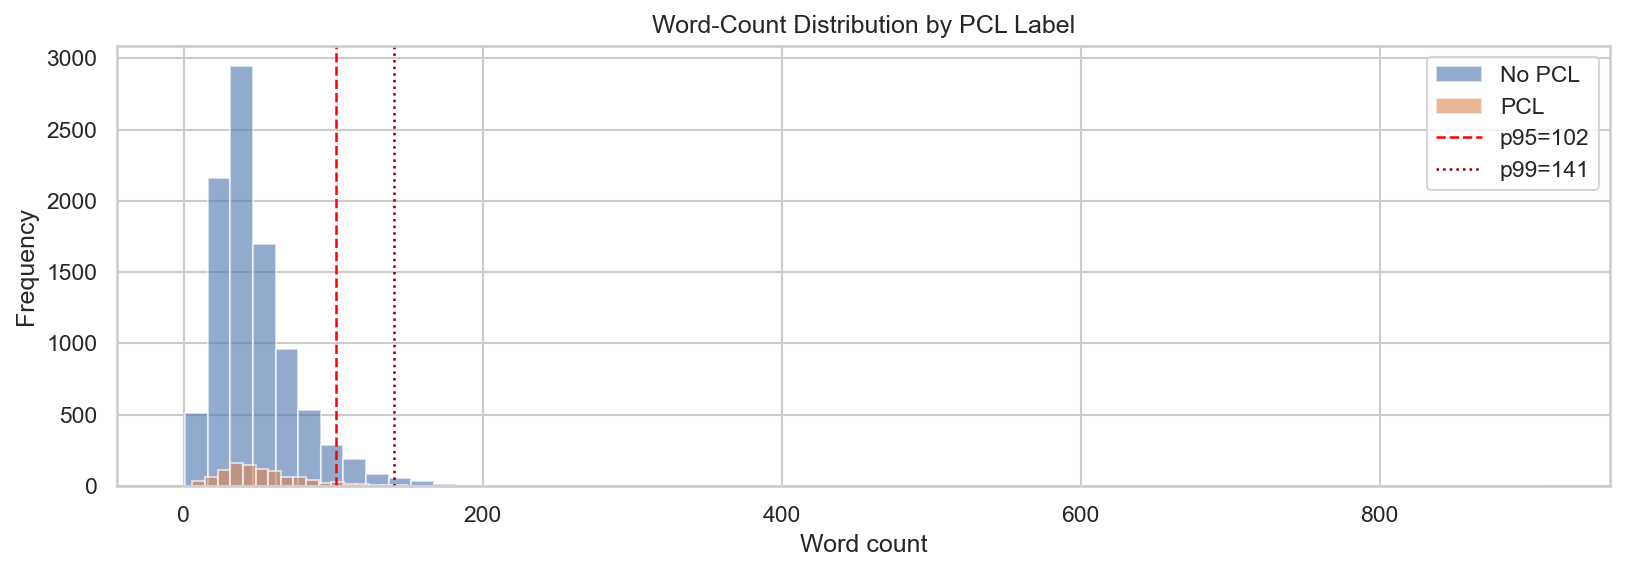
\includegraphics[width=0.85\textwidth]{figures/wordcount_distribution.png}
    \caption{Word-count distribution per class with p95 and p99
    cut-offs.}\label{fig:wordcount}
\end{figure}

\subsubsection{Findings}

The dataset is heavily class-imbalanced: 91\% of labelled paragraphs are
non-PCL, yielding a No-PCL\,:\,PCL ratio of roughly 9.5\,:\,1 (PCL accounts for
$\sim$9.5\% of the corpus).  The PCL class has a notably higher TTR (0.160
vs.\ 0.068), indicating greater lexical diversity per token, consistent with the
more varied rhetorical strategies used to express condescending language.
Furthermore, this PCL rate is not uniform across communities: an analysis of PCL
density reveals that `in-need' and `homeless' have much higher PCL span counts
than `immigrant', for example.

Paragraph lengths are right-skewed: the median is around 45 words, but the 95th
and 99th percentiles reach approximately 102 and 141 words respectively.

A scan found no exact text duplicates and no train-dev leakage in the official
splits.  Noise artefacts (HTML entities, non-ASCII characters, consecutive
spaces) are present in a small fraction of paragraphs ($<$2\%), with no URLs
detected.

\subsubsection{Impact on Modelling}

\textbf{Class imbalance.}  A na\"\i ve classifier predicting ``No PCL'' always
would achieve $\sim$91\% accuracy, making accuracy a misleading metric. Binary
F\textsubscript{1} on the PCL class must be the primary evaluation criterion,
and inverse-frequency class weights (or focal loss) should be applied during
training to avoid the model collapsing to the majority class.

\noindent\textbf{Sequence length.}  The p95 of 102 words maps to roughly
130--140 subword tokens for RoBERTa; the p99 of 141 words maps to $\sim$185
tokens. Setting \texttt{max\_length=256} therefore covers the entire practical
length distribution with comfortable headroom, while remaining half the cost of
512. A safe default is \texttt{max\_length=256} with truncation.

\noindent\textbf{Noise.}  The low artefact rate means aggressive cleaning is
unnecessary and risks removing meaningful content; simple whitespace
normalisation is sufficient.

\subsection{Technique 2: Lexical Analysis (N-gram Frequency \& Log-Odds)}

\subsubsection{Visual/Tabular Evidence}

Figures~\ref{fig:unigrams} and~\ref{fig:bigrams} show the top-20 unigrams and
bigrams per class after English stop-word removal.
Figure~\ref{fig:logodds} shows the 15 unigrams most enriched in each class by
log-odds ratio.

\begin{figure}[H]
    \centering
    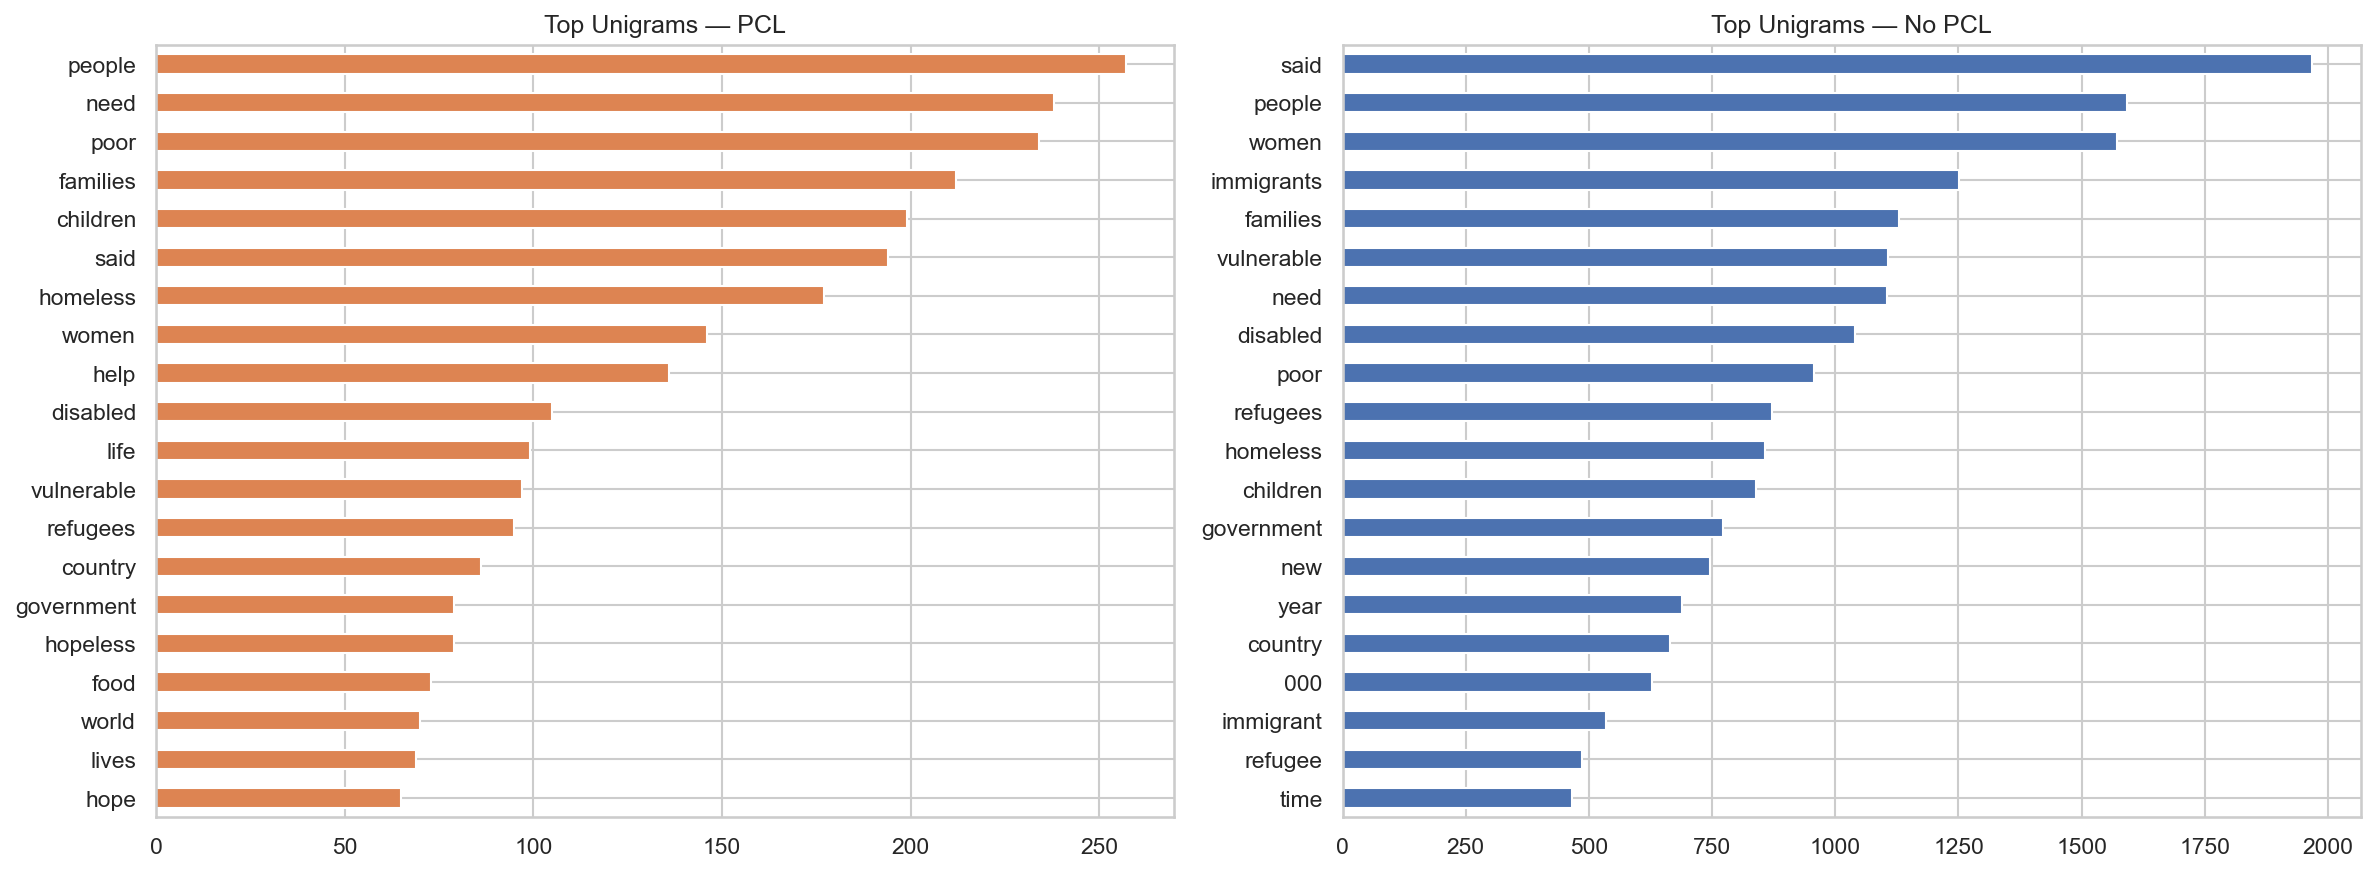
\includegraphics[width=\textwidth]{figures/unigrams.png}
    \caption{Top-20 unigrams in PCL (orange) and No-PCL (blue) paragraphs.}\label{fig:unigrams}
\end{figure}

\begin{figure}[H]
    \centering
    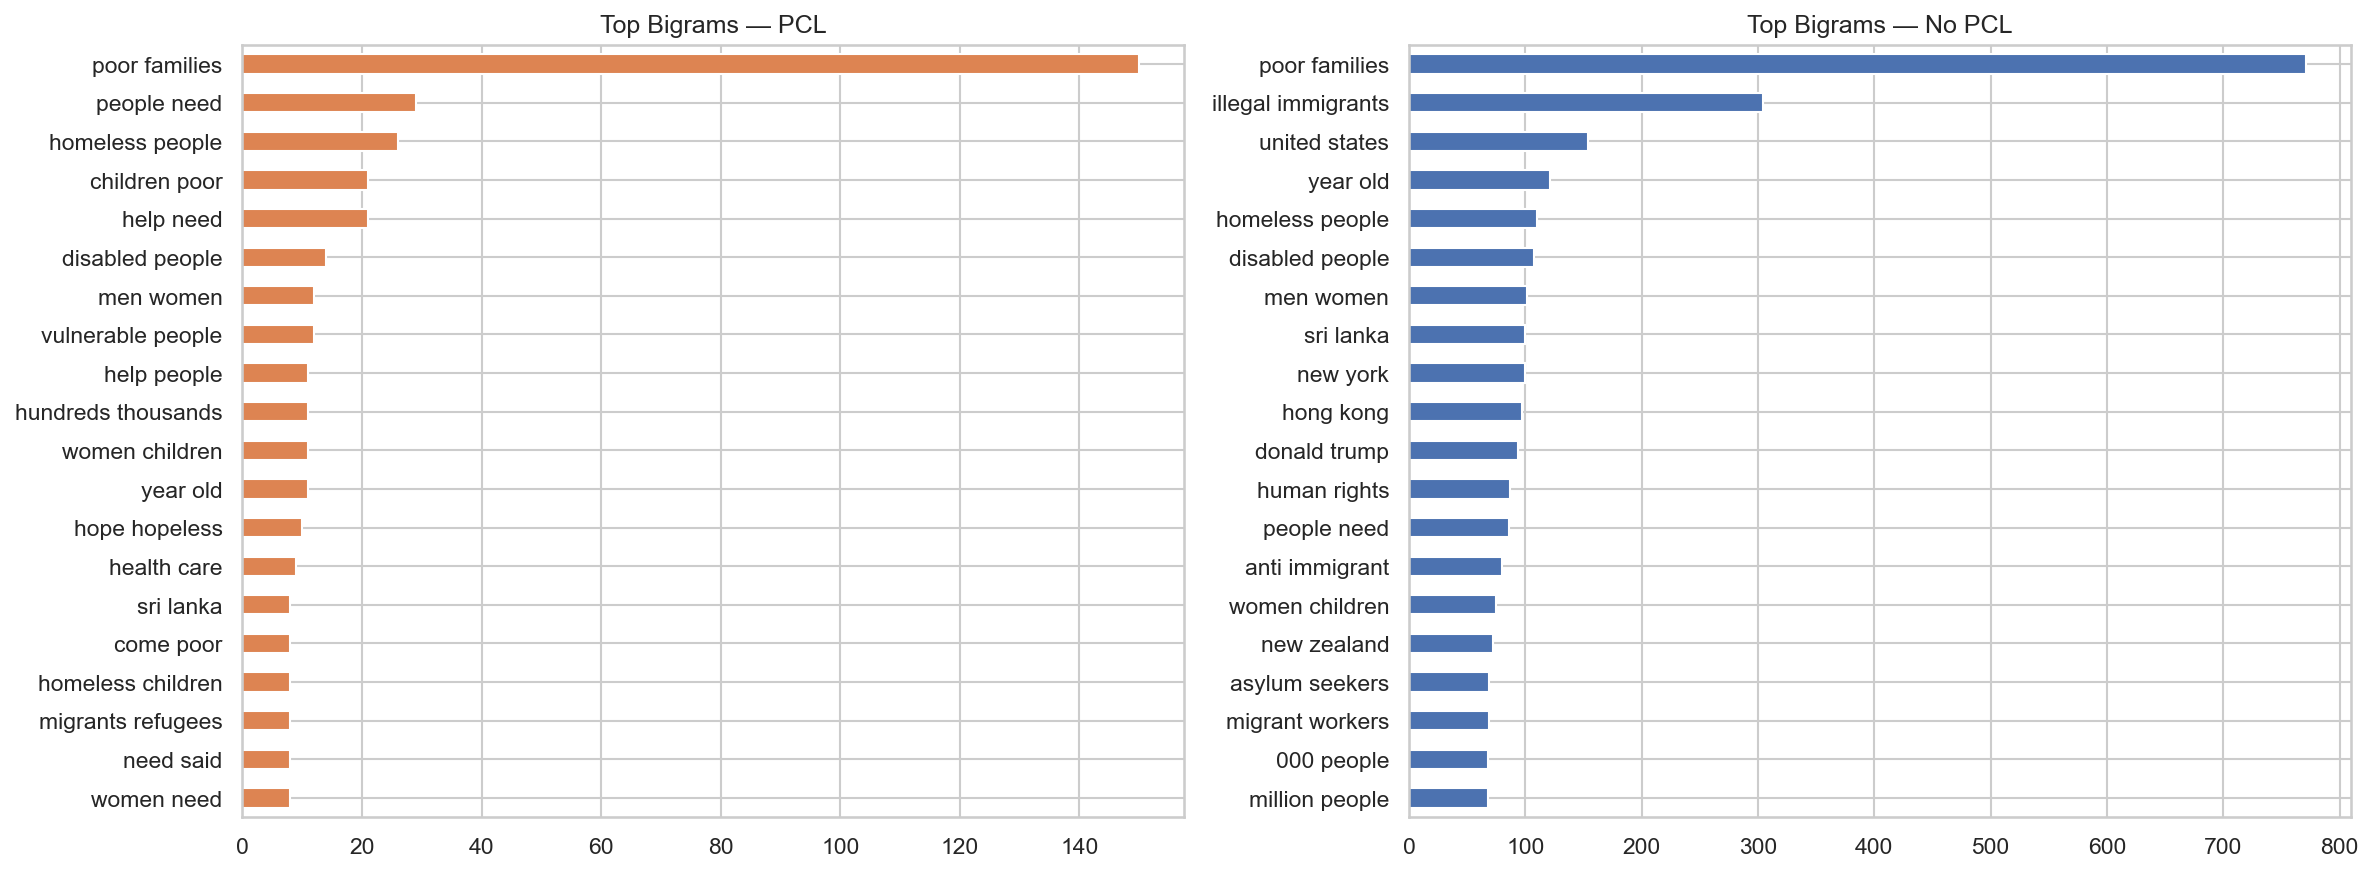
\includegraphics[width=\textwidth]{figures/bigrams.png}
    \caption{Top-20 bigrams in PCL (orange) and No-PCL (blue) paragraphs.}\label{fig:bigrams}
\end{figure}

\begin{figure}[H]
    \centering
    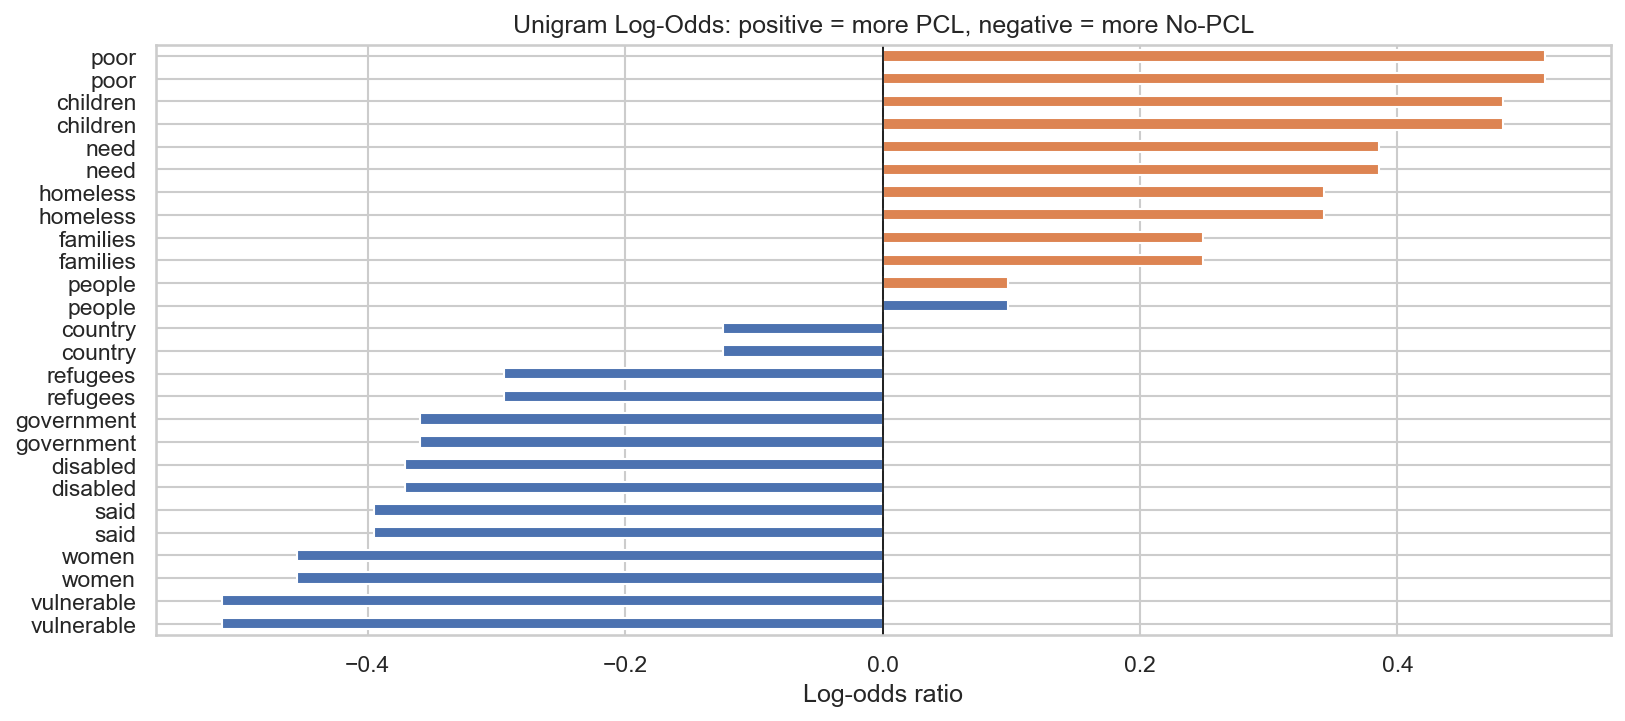
\includegraphics[width=0.85\textwidth]{figures/log_odds.png}
    \caption{Per-class unigram log-odds ratio; positive values indicate
             over-representation in PCL, negative in No-PCL.}\label{fig:logodds}
\end{figure}

\subsubsection{Findings}

Both classes share many high-frequency words (\textit{people, said, year}),
confirming that surface term frequency alone gives little signal.  The log-odds
analysis is more informative: PCL paragraphs are enriched with emotionally
loaded and othering terms (\textit{little, help, poor, children, lives, hope})
and phrases like ``living in poverty'' and ``the poorest'', directly reflecting
the dataset's PCL categories of \textit{poverty} and
\textit{over-generalisation}.  No-PCL paragraphs are enriched with neutral
reporting language (\textit{government, health, percent, new}).  The overlap in
the most frequent terms illustrates that PCL is driven by framing and semantic
context rather than lexical presence alone.

Critically, the n-gram distribution is not uniform across search keywords:
communities such as \textit{homeless} and \textit{in-need} contribute
disproportionately many high-PCL paragraphs, while keywords like
\textit{immigrant} are predominantly non-PCL.  This creates a direct risk of
label leakage via keyword identity: a model trained without controlling for
keyword distribution could learn to predict ``PCL'' simply because the keyword
\textit{homeless} appears, rather than due to any genuine condescension in the
text.

\subsubsection{Impact on Modelling}

\textbf{No keyword shortcuts.}  Because discriminative words (\textit{poor,
help, children}) also appear frequently in non-patronising contexts, a
bag-of-words classifier will struggle.  This motivates using a contextual model
(e.g., RoBERTa) that encodes the surrounding sentence rather than isolated
terms.

\noindent\textbf{Keyword-stratified splitting.}  The uneven PCL rate across communities
poses a concrete risk of label leakage.  To prevent the model learning
community-specific shortcuts rather than semantic condescension, the internal
validation split should be stratified on keyword in addition to label.  This
ensures every keyword appears in both train and internal-dev folds, forcing the
model to generalise across communities rather than memorising the PCL rate of a
particular group.

\noindent\textbf{Sequence length.}  Combining the finding from Technique~1 with the
contextual nature of PCL, \texttt{max\_length=256} is adopted.  The p99 of 141
words ($\sim$185 RoBERTa subword tokens) fits well within this budget, ensuring
no paragraph in the labelled corpus is truncated in practice, while keeping
memory cost well below the 512-token alternative.

% --------------------------------------------------------------------
\section{Exercise 3: Baseline and Proposed Approach (Stage
3)}\label{sec:proposed_approach}

\subsection{Proposed Approach}
The baseline fine-tunes RoBERTa-base~\cite{liu2019roberta} with standard cross-entropy and no
imbalance handling ($F_1{=}0.48$). Our model makes five changes.

\noindent\textbf{(1) DeBERTa-v3-base encoder~\cite{he2021debertav3}.} Disentangled attention
encodes content and position separately, consistently outperforming RoBERTa-base on
classification benchmarks.

\noindent\textbf{(2) Focal loss ($\gamma{=}2$).} $\mathcal{L} =
\frac{1}{N}\sum_i \alpha_{t_i}(1-p_{t_i})^2\,\mathrm{CE}(\log p_i, y_i)$, where
$\alpha_1{=}\sqrt{N_0/N_1}\approx3\times$ is applied as a separate per-sample
scalar (not via \texttt{cross\_entropy(weight=)}, which double-compensates). The
focal factor is \emph{not detached}; detaching creates a degenerate fixed point
at $p\approx0.41$ (verified analytically), causing $F_1{=}0$ throughout
training.

\noindent\textbf{(3) Prior bias init.} Classifier bias initialised to
$[0,\log(N_\text{PCL}/N_\text{NoPCL})]\approx[0,-2.2]$, anchoring $p(\text{PCL})\approx0.095$
at step~0 so focal gradients are correctly scaled from the first update.

\noindent\textbf{(4) Layer-wise LR decay (LLRD, $\lambda{=}0.9$).}
$\mathrm{lr}_k=\mathrm{lr}_\text{base}\times0.9^{L+1-k}$: the head trains at the full
$2\times10^{-5}$; embeddings at $\approx5\times10^{-6}$, preserving pre-trained representations.

\noindent\textbf{(5) Cosine schedule, keyword-stratified split, in-memory best-model tracking.}
A 6\,\% warmup (113 steps) clears the ramp before the epoch-1 checkpoint (step~235), followed
by cosine decay. The training set ($N{=}8{,}839$) is split 90/10 stratified by label and keyword.
\texttt{BestF1Callback} snapshots \texttt{model.state\_dict()} on each val-$F_1$ improvement
(patience~5) and restores it before evaluation. Training: effective batch~32
(16$\times$grad-accum~2), \texttt{max\_length=256}, up to 8 epochs.

\subsection{Rationale and Expected Outcome}
The 9.5\,:\,1 imbalance draws cross-entropy models toward the majority class; focal loss with
$\sqrt{\text{inverse-frequency}}$ weights addresses this, and the prior bias init ensures
correct gradient scaling from step~0. DeBERTa-v3-base's disentangled attention better encodes
the relational framing of PCL without the overfitting risk of larger variants
(Section~\ref{sec:paper_review}). LLRD protects lower-layer representations critical for this
pragmatics-heavy task. Keyword stratification prevents the model from learning community-specific
PCL rates rather than genuine condescension. Together these five changes are expected to yield
a dev-set $F_1$ meaningfully above~0.48.

\section{Exercise 4: Proposed Approach Implementation (Stage
4)}\label{sec:implementation}

Repository link on front page.

% --------------------------------------------------------------------
\section{Exercise 5: Evaluation and Error Analysis (Stage
5)}\label{sec:local_evaluation}

\subsection{Global Evaluation}
Omitted since results were not as expected; see next section for analysis.

\subsection{Local Evaluation}

Table~\ref{tab:results} summarises performance on the official dev set (2,094
paragraphs).

\begin{table}[H]
\centering
\begin{tabular}{lccc}
\toprule
Model & Precision & Recall & $F_1$ (PCL) \\
\midrule
Baseline (RoBERTa-base, CE)        & ---   & ---   & 0.579 \\
Proposed (DeBERTa-v3-base, Focal)  & 0.000 & 0.000 & 0.000 \\
\bottomrule
\end{tabular}
\caption{Dev-set results. Baseline exceeded its reported 0.48; proposed model
collapsed.}\label{tab:results}
\end{table}

The proposed model degenerated into a constant \emph{No PCL} predictor (90.5\,\%
accuracy, 0 true positives, 199 false negatives). The root cause is that
\texttt{BestF1Callback} never recorded a positive val $F_1$, so
\texttt{restore\_best()} was a no-op and the saved checkpoint reflects the fully
collapsed state.  Likely contributors: (1)~the base LR of $2\times10^{-5}$ is
too aggressive for DeBERTa-v3-base on a small dataset --- the original paper
recommends $5\text{--}9\times10^{-6}$; (2)~the $\sqrt{\text{inverse-frequency}}$
class weight ($\approx3\times$) may be insufficient to overcome the 9.5\,:\,1
majority-class gradient pressure at batch size 32; (3)~the five changes were not
validated jointly before full training.

Given more time the priorities would be: reduce LR to $5\times10^{-6}$; raise
the class-weight exponent to 0.75; add a 2-epoch sanity check monitoring mean
$p(\text{PCL})$ before committing to full training; and introduce deviations one
at a time to isolate any instability. The baseline result ($F_1{=}0.579 > 0.48$
reported) confirms the evaluation pipeline is correct.


\bibliographystyle{plain}
\bibliography{references} % Create references.bib as needed

\end{document}
